 %%%%%%%%%%%%%%%%%%%%%%%%%%%%%%%%%%%%%%%%%%%%%%%%%%%%%%%%%%%%%%%%%%%%
%%%%%%%%%%%%%%%%%%%%%%%%%%%%%%%%%%%%%%%%%%%%%%%%%%%%%%%%%%%%%%%%%%%%
% BSS Seminar Paper Template 
% © Fynn Lohre 
%
% In case of any questions, reach out to: VARFynn@gmail.com.
%
%%%%%%%%%%%%%%%%%%%%%%%%%%%%%%%%%%%%%%%%%%%%%%%%%%%%%%%%%%%%%%%%%%%%
%%%%%%%%%%%%%%%%%%%%%%%%%%%%%%%%%%%%%%%%%%%%%%%%%%%%%%%%%%%%%%%%%%%%


%------------------------------------------------------------------%
% 1. Required Packages
% Add packages and, additonally, customize included ones.
%------------------------------------------------------------------%

\documentclass[12pt,a4paper]{article}
\usepackage[
	left 	= 2.5cm,
	right 	= 2.5cm, 
	top 		= 2.5cm,
	bottom 	= 2.5cm,
]{geometry}
\usepackage[utf8]{inputenc}
\usepackage[english]{babel}
\usepackage[OT1]{fontenc}
\usepackage{amsmath}
\usepackage{amsfonts}
\usepackage{mathtools}
\usepackage{graphicx}
\usepackage{caption}
\usepackage[round]{natbib}
\usepackage{titlesec,xcolor}
\usepackage[hidelinks]{hyperref}
\hypersetup{
	colorlinks = true,
	urlcolor   = blue,
	linkcolor  = black, 
	citecolor  = blue, 
}
\newcommand{\mylink}[2]{\hyperref[#1]{\textcolor{blue}{#2}}}
% This allows you to link e.g. to figures: \mylink{F:2}{Figure 2}

\usepackage{fancyhdr}
\pagestyle{fancy}

% Formatting of the Sections has to be customized here
\usepackage{titlesec,xcolor}
\titleformat{\section}{\bfseries}{\thesection}{0.5em}{}
\titlespacing{\section}{0pt}{3ex plus 1ex minus 0.2ex}{10pt}
\setlength{\headheight}{14.49998pt}

\titleformat{\subsection}{\bfseries}{\thesubsection}{0.5em}{}
\titlespacing{\subsection}{0pt}{3ex plus 1ex minus 0.2ex}{10pt}
\setlength{\headheight}{14.49998pt}


%------------------------------------------------------------------%
% 2. Customizables
%------------------------------------------------------------------%
% Insert Name
\newcommand{\myname}{Fynn Lohre}

% Insert Title
\newcommand{\mytitle}{Bad Air Day: The Influence of Air Pollution on Quarterbacks' Performance - Evidence from the NFL}

% Insert Examiner
\newcommand{\myexaminer}{Professor Timo Hener, Ph.D. }

% Insert Course
\newcommand{\mycourse}{5440: Environmental Economics}

% Insert Submission Date
\newcommand{\mysubmission}{15.12.2023}

% Insert Matricle Nr. 
\newcommand{\mymatr}{202300181}

% Insert a "Display Name" of your paper (will be shown on the l.h.s. 
% of a certain page) - e.g. Doe 2014
\newcommand{\mypaper}{Lohre, 2023}



% If you want, you can customize the header
\author{\myname}
\title{\mytitle}
\lhead{\slshape \mypaper}
\chead{}
\rhead{\slshape \nouppercase{\leftmark}}


%------------------------------------------------------------------%
% 3. Content 
%------------------------------------------------------------------%
\begin{document}

%------------------------------------------------------------------%
% 3.1. Title Page
%------------------------------------------------------------------%
\begin{titlepage}
\center
\vfill

\includegraphics[scale=0.90]{BSS.png}
\vfill
\begin{tabular}[t]{lc}
Course:  & \mycourse \\
Examiner: & \myexaminer \\
Submission date: & \mysubmission \\
\end{tabular}
\vfill
{\large \textbf{\mytitle}}
\vfill
by \\ \vspace{3mm}
{\Large \myname}\\
(Student number \mymatr)\
\vfill
The relevant Data and Code are publicly available at \url{https://github.com/VARFynn/University_Contributions/tree/main/01_Master/02_Paper/Environmental_Econ_Paper}\\ 
\href{https://github.com/VARFynn/University_Contributions/tree/main/01_Master/02_Paper/Environmental_Econ_Paper}{
\includegraphics[scale=0.015]{GitHub.png}}
\vfill 
\scriptsize \textbf{Disclaimer}: The ''Bad Air Day'' catching phrase was independently created. During the research process, I serendipitously discovered two other papers with similar phrases. This resemblance was unintentional.
\vfill
\thispagestyle{empty}
\pagebreak
\end{titlepage}

%------------------------------------------------------------------%
% 3.2. Abstract
%------------------------------------------------------------------%
\newcounter{savepage}
\pagenumbering{roman}
\thispagestyle{empty}
\begin{abstract}
\textit{Insert Your Abstract here. } 
\end{abstract}
\clearpage

%------------------------------------------------------------------%
% 3.3. TOC + Content
%------------------------------------------------------------------%
\thispagestyle{plain}
\tableofcontents
\clearpage
\addcontentsline{toc}{section}{List of Tables}
\listoftables
\addcontentsline{toc}{section}{List of Figures}
\listoffigures
\pagebreak
\setcounter{savepage}{\arabic{page}}
\pagenumbering{arabic}
\section{Introduction}
In our modern world characterized by rapid industrialization and urbanization, the menace of airborne particulate matter, specifically PM10 and PM2.5, has risen to prominence as a pressing concern for environmental quality and human well-being. However, despite their increasing significance, PM10 and PM2.5 remain largely imperceptible to our senses, leading to their subtle but often underestimated influence on our daily lives and the environments we inhabit.
\clearpage
\section{Theoretical Framework}
While the exact physical processes and long-term effects of poor air quality are not precisely understood, a substantial body of literature exists showing correlations with various outcomes and potential causal linkages w.r.t. short-term effects. When referring to air pollutants, it is mostly referred to carbon monoxide (CO), sulfur dioxide (SO2), nitrogen oxide (NOx), ozone (O3) and particulate matter (PM). These particulate matter components, including PM10, PM2.5, and even ultrafine PM0.1, encompass a diverse range of particles, such as dust from various sources, smoke, but also pollen. As a significant driver of these pollutants (with the exception of SO2), traffic plays a crucial role (see e.g. \citealp{thorpe2008,costa2017,zhong2017} and also in \citealp{bauernschuster2017}), especially attributable to the impact of trucks \citep{lena2002}, airplanes \citep{schlenker2016} as well as diesel-fueled vehicles \citep{kinney2000}.

Consequently, for any mitigation policies, the damage curve of these pollutants must be more precisely understood. The occurring damages reach from direct health (e.g. \citealp{schlenker2016,kampa2008,chen2021}) towards indirect health effects like mental disorders (e.g. \citealp{pedersen2004,szyszkowicz2007,zhang2017}) as well as general life satisfaction (e.g. \citealp{mackerron2009,rehdanz2008,szyszkowicz2007}).  It is additionally evident that this primarily, but not only, affects children \citep{beatty2014} as well as older individuals (mediated through various predispositions; \citealp{peled2011}) and that the threshold for serious effects is substantially below the originally anticipated and by states set target level \citep{beelen2014}. Furthermore, long term exposures, as described in \citet{beelen2014}, as well as lagging effects (e.g. visible in effects onto infant's mortality based on the mother's exposure; \citealp{chay2003}) seem to additionally exist.

Apart from the personal hardships and financial costs associated with health challenges, it is indispensable to recognize these issues directly affecting work performance and, hence, the labor market in a tangible way. It not only impacts immediate wages at the individual level but is likewise manifested in broader welfare losses. Primarily, a decline in labor market participation is evident, attributed to absences resulting from illness (causally identified at least in Nordic countries; \citealp{hansen2000} \& \citealp{jans2018}). Secondarily, the phenomenon of presenteeism leads to further welfare losses. Despite being physically present at work, individuals grappling with health issues could contribute to an overall decline in productivity \citep{zivin2012}. While \citet{zivin2012} focus on the productivity of fruit harvesters and, hence, solely on the physical layer of health effects, it remains open if a cognitive layer additionally exists. This appears plausible as cognitive effects (see e.g. \citealp{schikowski2015,tonne2014,ranft2009}) as well as general changes in decision making \citep{archsmith2018} caused by higher pollution levels appear likely. As the nature of work undergoes a transformation from routine and manual labor to tasks demanding greater cognitive engagement, the importance of this cognitive layer
is poised to grow.

Given the prevalent issue of limited firm level data availability, scholars often turn to athletes' performances due to the accessibility and comprehensiveness of the data they offer. Nevertheless, when examining these athletes, particularly concerning their sensitivity to air pollution, it is crucial to understand its caveat. As athletes are on of the least vulnerable individuals due to their high level of fitness (see the previous argument of \citealp{peled2011}),  estimates derived must consequently be regarded as conservative or lower-bound estimations. The causal identification of \citet{lichter2017} w.r.t. soccer showing a significant decrease in passed played (and, hence, productivity) induced through exogenous PM10 variation should, therefore, be considered a lower bound productivity decrease. \citet{lichter2017}, however, solely focus on the existence of physical effects, disregarding a possible (further) cognitive layer. Still, their identification setups validly allows to exploit the exogenous variation in air pollution. The results further support similar, less  rigorous results, like negative correlations with performance of Olympic marathon runners \citep{marr2010} or Chinese soccer players \citep{qin2022}. Conversely, while \citet{heintz2022} primarily focus on the cognitive dimension for NFL and MLB players without employing a robust identification strategy, their significant results imply the potential existence of a lower bound estimate. 

Accordingly, this project report combines a rigorous identification framework similar to \citet{lichter2017} with examining the cognitive productivity effects for quarterbacks in the NFL similar to \citet{heintz2022}. Essentially, this analysis hinges upon the assumption that \citeauthor{lichter2017}'s reported physical productivity decrease uniformly affects all players. Without this assumption, the examination lacks coherence and would require a comprehensive analysis incorporating general equilibrium considerations, including potential spillover effects from specific player positions onto others.

As a foundational step, this project delves into the causal linkage between PM10 - the largest particles - and quarterbacks' performance, as visible in the following hypothesis: \\[0.2cm]
\textbf{H I: Increased exposure to PM10 will lead to a reduction in quarterback performance. } \\[0.2cm]
The hypothesis implies that although quarterbacks undergo similar physical consequences stemming from PM10 exposure as their teammates, the distinct emphasis on cognitive functions within the quarterback role may lead to a decline in their on-field performance. As a robustness check, the Air Quality Index (AQI) displaying the highest value of among the group of pollutants is used. \\[0.2cm]
\textbf{H II: The closure of the stadium will mitigate any effect of PM10.} \\[0.2cm]
This hypothesis is based on the concept of mitigation strategies, a notion indirectly inferred from the findings in \citet{deschenes2017}. Specifically, it considers the significant impact of air conditioning, as detailed in the study by \citet{lin2013}, in reducing the effects of air pollution (and PM10). However, for closed stadiums, the situation is less straightforward: if there is an effect, it may imply that general air pollution levels during the day are influential. Conversely, a lack of effect in closed stadiums would support the idea that air pollution impacts are more direct and immediate in open environments.

This term paper, however, encounters a significant limitation rooted in the distinction between actual and perceived air pollution. A plethora of scholars highlight that individuals' perception of pollution can greatly influence their behavior and performance (e.g. \citealp{rehdanz2008,schumacher2008,mackerron2009,chiarini2020,gong2020,claeson2013}). This perceived pollution may not always be causally linked with actual pollution levels. Therefore, the study's reliance on objective pollution measurements may overlook the subjective experience of individual quarterbacks and eventually overestimating the effect linked to the pollutant itself.\footnote{If the correlation between pollutant and perception is large enough, this argument becomes less relevant from a policy perspective.}

\clearpage

\section{Data and Descriptive Statistics}
In order to tackle the research question, it is necessary to combine different data sets. These different sets of data are (i) NFL's official weekly statistics, (ii) pollution data from the United States Environmental Protection Agency (\citeauthor{EPA}) as well as (iii) the spatial climate dataset from the \citeauthor{PRISM}. 



\begin{table}[h]
  \centering
  \caption{Summary Statistics of Metric Variables}
  \label{tab:1}
  \begin{tabular}{lrrrrr}
    \hline \hline
    Variable & Obs & Mean & Std. dev. & Min. & Max. \\
    \hline
    \textit{Quarterbacks' Performance} \\
    Rating & 7,095 & 88.47 & 27.83 & 0.00 & 158.30 \\
    Attempts & 7,095 & 32.29 & 10.33 & 5.00 & 68.00 \\
    Completions & 7,095 & 20.30 & 7.18 & 0.00 & 45.00 \\
    Completion Rate & 7,095 & 62.65 & 10.51 & 0.00 & 100.00 \\
    Yards & 7,095 & 231.05 & 87.84 & 0.00 & 527.00 \\
    Yards per Attempt & 7,096 & 7.19 & 1.97 & 0.00 & 17.00 \\
    Interceptions & 7,095 & 0.80 & 0.93 & 0.00 & 6.00 \\
    Interception Rate & 7,095 & 2.57 & 3.34 & 0.00 & 37.50 \\
    Touchdowns & 7,095 & 1.43 & 1.16 & 0.00 & 7.00 \\
    Touchdown Rate & 7,095 & 4.52 & 3.94 & 0.00 & 40.00 \\
    Passing Success Rate & 7,095 & 45.16 & 10.96 & 0.00 & 100.00 \\ [0.5cm]
    \textit{Pollution/Weather} \\
    PM10 (AQI value) & 7,095 & 20.59 & 14.86 & 0.00 & 171.00 \\
    Precipitation (mm) & 7,095 & 0.18 & 0.35 & 0.00 & 2.15 \\
    Temperature (°F) & 7,095 & 50.13 & 10.53 & 18.50 & 76.00 \\
    \hline \hline
  \end{tabular}
\end{table}

Initiating the exploration with the NFL's official weekly statistics, this dataset offers a comprehensive array of player-specific and game-related metrics for 7,095 individual performances of 222 different quarterbacks. To be precise, the data is initially scraped from NFL's Fantasy Football application and, afterwards, merged, cross-checked and enriched by data from \citeauthor{Stathead}. This leads to a set containing every single quarterback performance from the last 12 completed seasons. Therefore, a reasonable assumption can be made that neither measurement errors nor selection biases are present. By exclusively considering players with a minimum of $\geq 5$ passes, it is ensured that the sample per game is sufficient enough and the individuals primarily orchestrating plays are captured. Thus, in this project report, the term 'quarterback' is used inclusively, referring not solely to the conventional position but also acknowledging versatile players from other positions - in football terms the ''Taysom-Hill-Like-Players''. Another restriction imposed onto the data is the exclusion of games not played on American ground, the so called  international pathway games. This exclusion ensures a more uniform and consistent dataset, aligning with the aim of identifying a causal effect of air pollution, as it can not be assumed with certainty that those games comply to the same standards as regular NFL games. Finally, every performance is manually matched to the respective place/stadium\footnote{For the sake of completeness: This project respects geographical changes of franchises like the move from San Diego to L.A. for the Charges - see \mylink{AppF:1}{Appendix A}. However, the linked stadium names are not supposed to capture every name or minor location change (like a stadium next to the old one).}. 

For the remaining 7,095 distinct performances, the common metric measures of performance can be seen in \mylink{tab:1}{Table 1}. While most of them are self-explanatory, a precise explanation of the calculation is still necessary - even for die-hard football fans. The quarterback rating follows the specific calculation, 
\begin{equation}
Rating = \dfrac{CP + Y/A + TP + IP}{6} \times 100,
\end{equation}
whereas the percentages have already weights included in their calculation. The used completion percentage (CP) is $ ((\textrm{Completed Passes} / \textrm{Pass Attempts}) - 0.3) \times 5$, the yards per attempt (Y/A) are $((\textrm{Passing Yards} / \textrm{Pass Attempts}) - 3) \times 0.25$, the touchdown percentage (TP) is $(\textrm{Touchdown Passes} / \textrm{Pass Attempts}) \times 20$ and the interception percentage is  $(0.095 - (\textrm{Interceptions} / \textrm{Pass Attempts})) \times 25$. Thus, every rating is $ \in [ 0.00 ,158.30 ]$, with a higher rating describing a better overall performance weighting every usual performance dimension. Further, the passing success rate is 

\begin{equation}
\textrm{Passing Success Rate} = \dfrac{\textrm{Successful Passes}}{\textrm{Attempts} + \textrm{Sacks}},
\end{equation}
with a pass being considered successful if it gains 40 \% of the distance on first down, 60 \% on second down and 100 \% on third or fourth down. 

In order to access reliable data on PM10 concentration, the publicly available air quality data from the \citeauthor{EPA} is used. This data set contains every measured concentration pinned down to the respective station. Despite its recognized reliability, the \citeauthor{EPA} dataset does come with two caveats: missing data for some stations and its provision of solely daily average measurements. With the exception of three particular cases, stations selected are notably in close proximity to the stadium. Prioritizing the closest station ensures primary data selection, while in instances of missing data, the highest value among the given alternative stations, which are still in reasonable close proximity, is considered. For Seattle, Green Bay and Foxborough no reasonable close station measuring PM10 exists, which is why the next city with a station is chosen.\footnote{This might be a stretch. However, w.r.t. weather data a comparability seems reasonable. See tab ''Mapping'' in Football$\_$Data$\_$ FULL.xlsx for detailed mapping.}
In cases with persisting missing data, linear interpolation and as a robustness check an ARIMA model are applied to estimate missing values. While it results in similar final findings (w.r.t $\hat{\beta}$), it is crucial to recognize that it only serves as a ''second best approach''. The major assumption of a reasonable autocorrelation of the (missing) PM10 values is imposed. However, dropping missing values implicitly assumes the same autocorrelation as regressions only yield coefficients conditional one the inclusion condition. Hence, the coefficient is in both cases equally biased if the missing data is selectively excluding deviations from the trend. While adopting this second best approach may be the most plausible under this circumstances, it is essential to acknowledge that it rests on this fundamental assumption. Still, this method represents a compromise due to the unfeasibility of attaining complete data, which stands as the ideal but unattainable first-best solution.

The \citeauthor{EPA} dataset is reporting PM10 as its Air Quality Index (AQI) value, which is normally used to compare values from different pollutants to each other. The calculation is given in the respective technical assistance document of \citeauthor{EPA} as 

\begin{equation}
I_{PM10}= \dfrac{I_{HI}-I_{LO}}{BP_{HI}-BP_{LO}}(C_{PM10} - BP_{LO})+I_{LO}.
\end{equation}
I in that case is the index, C the truncated concentration (for PM10 it is truncated to an integer), 
$BP_{HI}$ ($BP_{LO}$) the concentration breakpoint that is greater (lower) than or equal to C and $I_{HI}$ ($I_{LO}$) the AQI value corresponding to $BP_{HI}$ ($BP_{LO}$, see \mylink{T:A1}{Appendix B} for a mapping of $\mu g/m^3$ on AQI). As visible in \mylink{F:1}{Figure 1} enough variation exists within and between locations. 
\begin{figure}[h]
	\center
	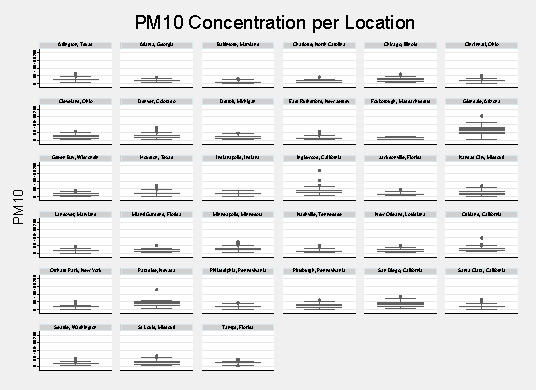
\includegraphics[scale=1.7]{../05_Figures/PM10_Concentration_per_Place.pdf}
	\caption*{\footnotesize \textit{Source: Own Visualization based on \citeauthor{EPA} Data. Note: It is essential to underscore that the displayed distributions are solely based on occurred match days and do not resemble the general distribution of the respective location. PM10 Concentration is measured in AQI.}}
	\addvspace{-0.6\baselineskip}
	\caption{Box Plot of PM10 Concentration per Location}
	\label{F:1}
\end{figure}

The dataset is completed with the implementation of weather controls from data gathered by the \citeauthor{PRISM} (Oregon State University). This includes the average daily temperature and daily precipitation (see \mylink{AppF:2}{Appendix B} for distribution per location). 


\section{Empirical Framework}
To investigate a potential causal linkage between air pollution and quarterbacks' performances, this term-paper utilizes an empirical framework effectively capturing both unobserved and observed heterogeneity. As visible in the following equation,
\begin{equation}
\hat{Y}_{ijkls} = PM10 \times \beta_l + {W'} \zeta_l + \alpha_i + \mu_{js} + \eta_{ks} + Away \times \delta + \varepsilon_{ijkls},
\end{equation}
the dependent measurement of performance ($\hat{Y}$) is segmented into five dimensions (i.e. i,j,k,l and s). This five-dimensional segmentation allows to remove time-invariant heterogeneity (i.e. $ \mu_{js} \wedge \eta_{ks}$) as well as individual-specific variation constant over time (i.e. $\alpha_i$). This already reveals that, $i \in Q$ (set of all quarterbacks), $\{s \in \mathbb{Z} \, | \, 2010 \leq s \leq 2022\}$, $j \in T$ (set of teams) and $k \in O$ (set of opponents). Exemplifying the concept, $\hat{Y}_{ijkls}$ encapsulates the estimated performance of a quarterback ($i$) within a designated team ($j$), operating against a distinct defensive unit ($k$) during a specified season ($s$) in a specific stadiumtype ($l$). 

Consequently, $\mu_{js}$ is the vector of team (offense) by season and $\eta_{ks}$ the vector of opponent (defense) by season fixed effects. Notably, within the NFL, a significant portion of variation can be attributed to changes on a season basis, including transitions like alterations in offensive and defensive coordinators, playbook changes, player acquisitions, and related dynamics. Furthermore, the strategic practice of teams 'tanking' in specific seasons to gain advantageous draft positions highlights the necessity of employing the mentioned seasonal fixed effects to comprehensively address the diverse but unobserved factors impacting team's and, hence, quarterback's performance. In light of these considerations, additionally including the quarterback-specific effect\footnote{In a pre-check, I do not find any evidence w.r.t. to a season by quarterback variation, which is not already captured in $\mu_{js}$. The same holds for any age variation as deployed by \citet{heintz2022}.}, which encompasses general playstyle, leads to a robust identification framework that effectively accounts for nearly all non-random variation in performance. In spite of this, it's crucial to recognize that while this model covers a wide range of unobserved factors, it does not preclude the presence of additional effects on specific game days, e.g. minor injuries. These effects are considered to follow a poisson distribution (Pois({$\lambda$)) with the same probability to occur for defense and offense (i.e. $Pr_j(X=x) = Pr_k(X=x)$) and being orthogonal to the primary marginal effect of interest. Hence, it can be considered non-influential w.r.t. causal inference, as it just leads to more noise not affecting the primary effect.\footnote{Generally, this is a strong assumption to make. However, any correlation between $\varepsilon_{ijks}$ and $\Delta PM10$ seems highly unlikely given the data.} The model's setup is completed with a dummy for having an away performance as well as ${W'}$, the matrix weather controls by stadiumtype, encompassing temperature and precipitation.

Proceeding to investigate the marginal effect of interest, denoted as $\hat{\beta}$, it is therefore appropriate to frame this analysis a causal one.  Incorporating it as an interaction term with stadiumtype $l \in \{$Open, Closed, Retractable$\}$ allows to estimate three distinct average marginal effects, i.e. $\hat{\beta}_{open},\hat{\beta}_{closed} \wedge \hat{\beta}_{retractable}$. Given the hypothesis, $\hat{\beta}_{open}$ is supposed to significantly differ from zero, if it were a causal relationship between PM10 and the respective $Y$, as no direct mitigation is possible. W.r.t. $\hat{\beta}_{closed} \wedge \hat{\beta}_{retractable}$ several effects are ex ante conceivable. In a closed stadium, both a non-significant as well as a positive, but less nuanced, effect would align with theory. The former aligns with parts of the literature suggesting a immediately (short-term)  observable effect, whereas the latter corresponds to theory implying an effect resulting from prolonged exposure. In a correct specified model, the effect should, however, never be positive, i.e. increasing performance. In the context of a retractable stadium, a dynamic interplay between closure and PM10 exposure could even lead to positive effect, when the closure is a mitigation response to high PM10 concentrations. Given this reasoning, it appears plausible that the latter $\hat{\beta}$ demonstrates orthogonality with the error term. Hence, the identification emphasis tilts more decisively towards analyzing $\hat{\beta}_{open} \wedge \hat{\beta}_{closed}$.

The dependent performance measure is..

\clearpage \section{Results and Discussion}
\begin{table}[!htbp] \centering 
  \caption{Effect of PM10 on Quarterbacks' Performance (Attempts, Yards, Interceptions)} 
  \label{T2} 
\begin{tabular}{@{\extracolsep{5pt}}lccc} 
\\[-1.8ex]\hline 
\hline \\[-1.8ex] 
 & \multicolumn{3}{c}{\textit{Dependent Variable:}} \\ \cline{2-4} \\ [-1.8ex]
 & Attempts & Yards & Interceptions \\ 
  & (1) & (2) & (3)\\ \hline \\[-1.8ex] 
 \underline{\textit{Average Marginal Effect PM10}}\\[0.4cm]
  $\hat{\beta}_{closed}$& 0.0008 & -0.0776 & -0.0028 \\ 
  & (0.0236)  & (0.2033)& (0.0025) \\[0.4cm]
  $\hat{\beta}_{open}$& -0.0281$^{**}$ & -0.1679 & -0.0026$^{*}$\\ 
  & (0.0137) & (0.1127) & (0.0014) \\[0.4cm]
  $\hat{\beta}_{retractable}$& -0.0053 & 0.0900 & -0.0014 \\ 
  & (0.0124) & (0.0994) & (0.0013)\\ [0.4cm]
  \underline{\textit{Controls}} \\[0.4cm]
  Offense $\times$ Season Fixed Effect & $\surd$ & $\surd$ & $\surd$ \\[0.4cm]
   Defense $\times$ Season Fixed Effect & $\surd$ & $\surd$  & $\surd$ \\[0.4cm]
    Quarterback Individual Effect & $\surd$ & $\surd$ & $\surd$  \\[0.4cm]
    Weather $\times $ Stadiumtype & $\surd$ & $\surd$ & $\surd$ \\[0.4cm]
    Away Performance & $\surd$ & $\surd$ & $\surd$\\
\hline \\[-1.8ex] 
Observations & 7,095 & 7,095 & 7,095 \\ 
R$^{2}$ & 0.3661 &  0.3981 & 0.1829\\ 
RMSE & 8.9059 & 73.817 & 0.9076\\ \hline 
\hline \\[-1.8ex] 
\multicolumn{4}{l}{\footnotesize \textit{Note:} The significance levels equal {$^{*}$p$<$0.1; $^{**}$p$<$0.05; $^{***}$p$<$0.01}.  Furthermore, robust} \\ \multicolumn{4}{l}{\footnotesize standard errors (HC1) are displayed. Values are rounded to four decimal places.}
  \end{tabular}
\end{table} 
\clearpage
\begin{table}[!htbp] \centering 
  \caption{Effect of PM10 on Quarterbacks' Performance (Completion Rate, Interception Rate \& Rating)} 
  \label{T1} 
\begin{tabular}{@{\extracolsep{5pt}}lccc} 
\\[-1.8ex]\hline 
\hline \\[-1.8ex] 
 & \multicolumn{3}{c}{\textit{Dependent Variable:}} \\ \cline{2-4} \\ [-1.8ex]
 & Success Rate & Interception Rate & Rating \\ 
  & (4) & (5) & (6)\\ \hline \\[-1.8ex] 
 \underline{\textit{Average Marginal Effect PM10}}\\[0.4cm]
  $\hat{\beta}_{closed}$& 0.0130 & -0.0052 & 0.0642 \\ 
  & (0.0277)  & (0.0080)& (0.0657) \\[0.4cm]
  $\hat{\beta}_{open}$&  0.0156 & -0.0063 & 0.0480\\ 
  & (0.0148) & (0.0049) & (0.0382) \\[0.4cm]
  $\hat{\beta}_{retractable}$& 0.0348 & -0.0039 & 0.0782$^{**}$\\ 
  & (0.0122) & (0.0042) & (0.0364)\\ [0.4cm]
  \underline{\textit{Controls}} \\[0.4cm]
  Offense $\times$ Season Fixed Effect & $\surd$ & $\surd$ & $\surd$ \\[0.4cm]
   Defense $\times$ Season Fixed Effect & $\surd$ & $\surd$  & $\surd$ \\[0.4cm]
    Quarterback Individual Effect & $\surd$ & $\surd$ & $\surd$  \\[0.4cm]
    Weather $\times $ Stadiumtype & $\surd$ & $\surd$ & $\surd$ \\[0.4cm]
    Away Performance & $\surd$ & $\surd$ & $\surd$\\
\hline \\[-1.8ex] 
Observations & 7,095 & 7,095 & 7,095 \\ 
R$^{2}$ & 0.3525 & 0.2338   &  0.3055 \\ 
RMSE & 9.5531 & 3.1676  & 25.1200 \\ \hline 
\hline \\[-1.8ex] 
\multicolumn{4}{l}{\footnotesize \textit{Note:} The significance levels equal {$^{*}$p$<$0.1; $^{**}$p$<$0.05; $^{***}$p$<$0.01}.  Furthermore, robust  standard} \\ \multicolumn{4}{l}{\footnotesize errors (HC1) are displayed. Values are rounded to four decimal places.}
  \end{tabular}
\end{table} 
\section{Summary and Concluding Remarks}
\clearpage


%------------------------------------------------------------------%
% 4. References
% Insert your .bib name here, then it will automatically generate
% Just cite the papers by \citep{}, \citet{} or \citealp{}
%------------------------------------------------------------------%
\pagenumbering{roman}
\setcounter{page}{\thesavepage}
\pagestyle{plain}
\addcontentsline{toc}{section}{References}
\bibliographystyle{apa}
\bibliography{EnvEcon.bib}
\clearpage

%------------------------------------------------------------------%
% 5. Appendix
%------------------------------------------------------------------%
\appendix
\section{Further Figures}
\begin{figure}[h]
	\center
	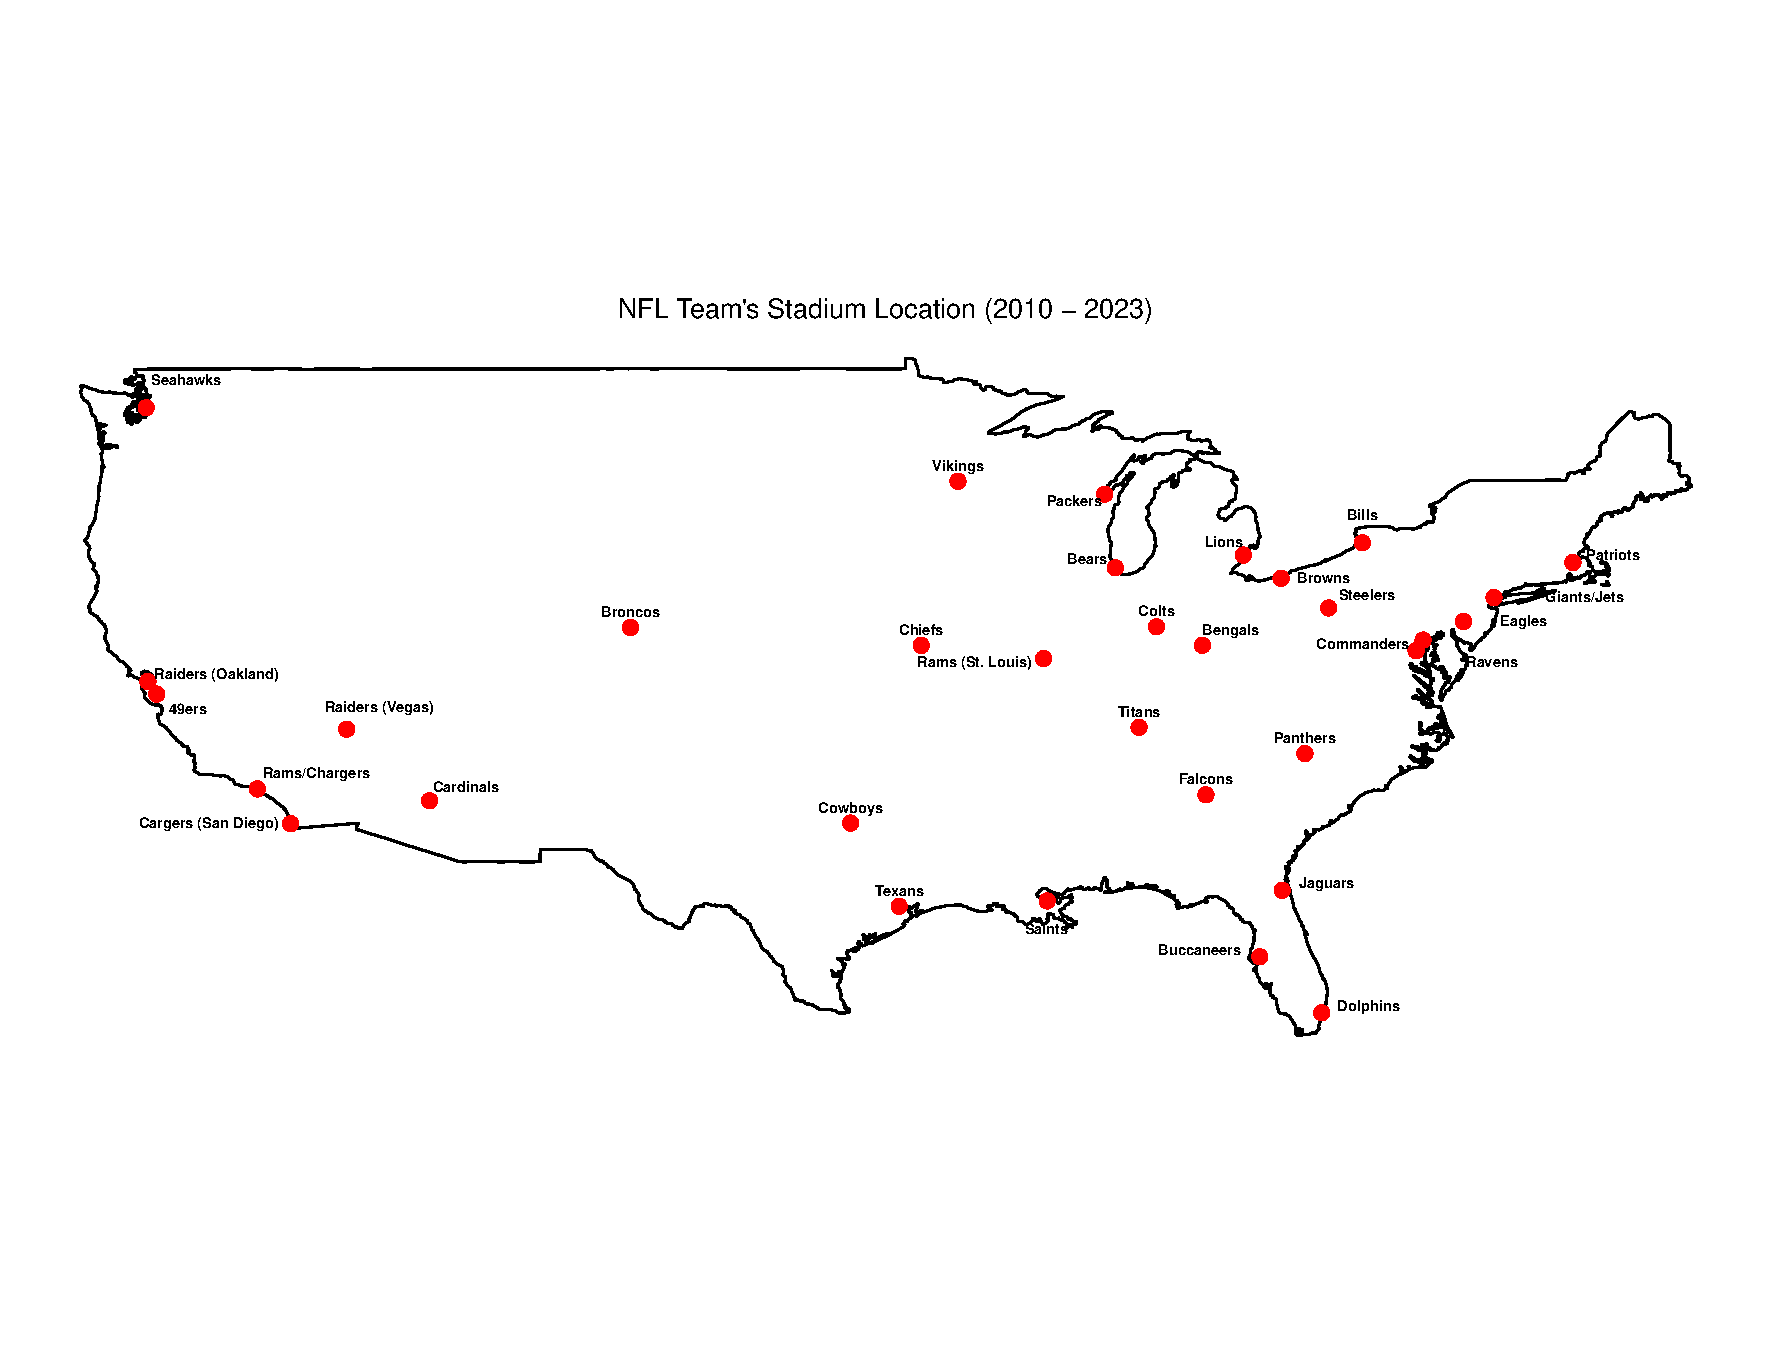
\includegraphics[scale=0.59, angle = 90]{../05_Figures/Teams_Location.pdf}
	\caption{Map of NFL Team's Stadium Locations in Sample}
	\addvspace{-0.6\baselineskip}
	\caption*{\footnotesize \textit{Source: Own Visualization.}}
	\label{AppF:1}
\end{figure}
\clearpage
\vfill
\begin{figure}
	\center
	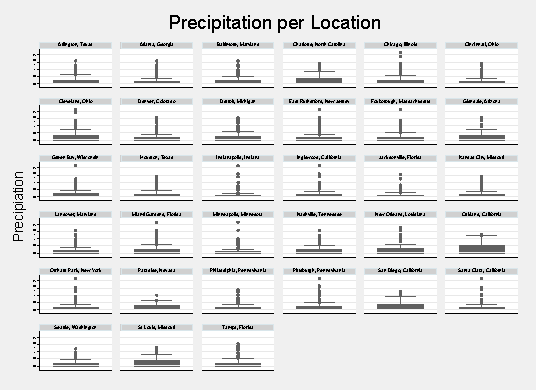
\includegraphics[scale=1.7]{../05_Figures/Percipitation_per_Place.pdf}
	\caption*{\footnotesize \textit{Source: Own Visualization based on \citeauthor{PRISM} Data. Note: It is essential to underscore that the displayed distributions are solely based on occurred match days and do not resemble the general distribution of the respective location. Precipitation is measured in mm.}}
	\addvspace{-0.6\baselineskip}
	\caption{Box Plot of Precipitation per Location}
	\label{AppF:2}
\end{figure}
\vfill
\clearpage
\vfill
\begin{figure}
	\center
	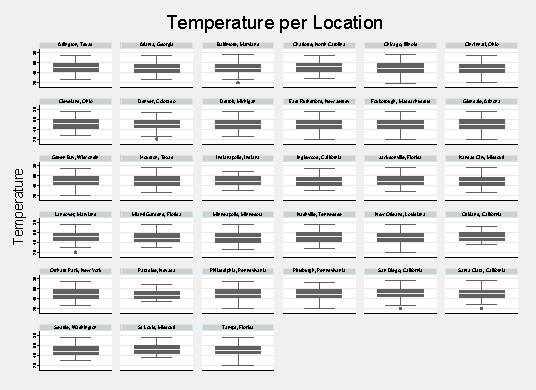
\includegraphics[scale=1.7]{../05_Figures/Temperature_per_Place.pdf}
	\caption*{\footnotesize \textit{Source: Own Visualization based on \citeauthor{PRISM} Data. Note: It is essential to underscore that the displayed distributions are solely based on occurred match days and do not resemble the general distribution of the respective location. Temperature is measured in Fahrenheit (°F).}}
	\addvspace{-0.6\baselineskip}
	\caption{Box Plot of Temperature per Location}
	\label{AppF:3}
\end{figure}
\vfill
\clearpage
\section{Further Tables}
\begin{table}[h]
 \caption{Mapping of AQI on PM10 Concentration Value} 
  \label{T:A1} 
\center \vspace{-0.5cm}
\begin{tabular}{|c|c|c|}
\hline
AQI & PM10 & Air Quality Category \\\hline
0 - 50 & 0 - 54 & Good \\
51 - 100 & 54 - 154 & Moderate \\
101 - 150 & 155 - 254 & Unhealthy for Sensitive Groups \\
151 - 200 & 255 - 354 & Unhealthy \\
201 - 300 & 355 - 424 & Very Unhealthy \\
301 - 400 & 425 - 504  & Hazardous \\
401 - 500 & 505 - 604 & Hazardous \\
\hline
\end{tabular}
\vspace{0.2cm}\caption*{Source: \citeauthor{EPA}}
\end{table}

\end{document}
